\section{\method: A Novel Memory Mechanism Tailored for LLMs}
\saveSpaceSec

In this section, we provide a detailed description of \method, our novel memory mechanism designed for LLMs. As shown in Fig. \ref{fig:framework}, \method is a unified mechanism structured around three central pillars: (1) a memory storage (\sect~\ref{sec:memorystorage}) serving as the primary data repository, (2) a memory retriever (\sect~\ref{sec:memoryretrieval}) for context-specific memory recollection, and (3) a memory updater (\sect~\ref{sec:memory-updater}) drawing inspiration from the Ebbinghaus Forgetting Curve theory, a time-tested psychological principle pertaining to memory retention and forgetting.
\begin{figure*}[t]
\begin{center}
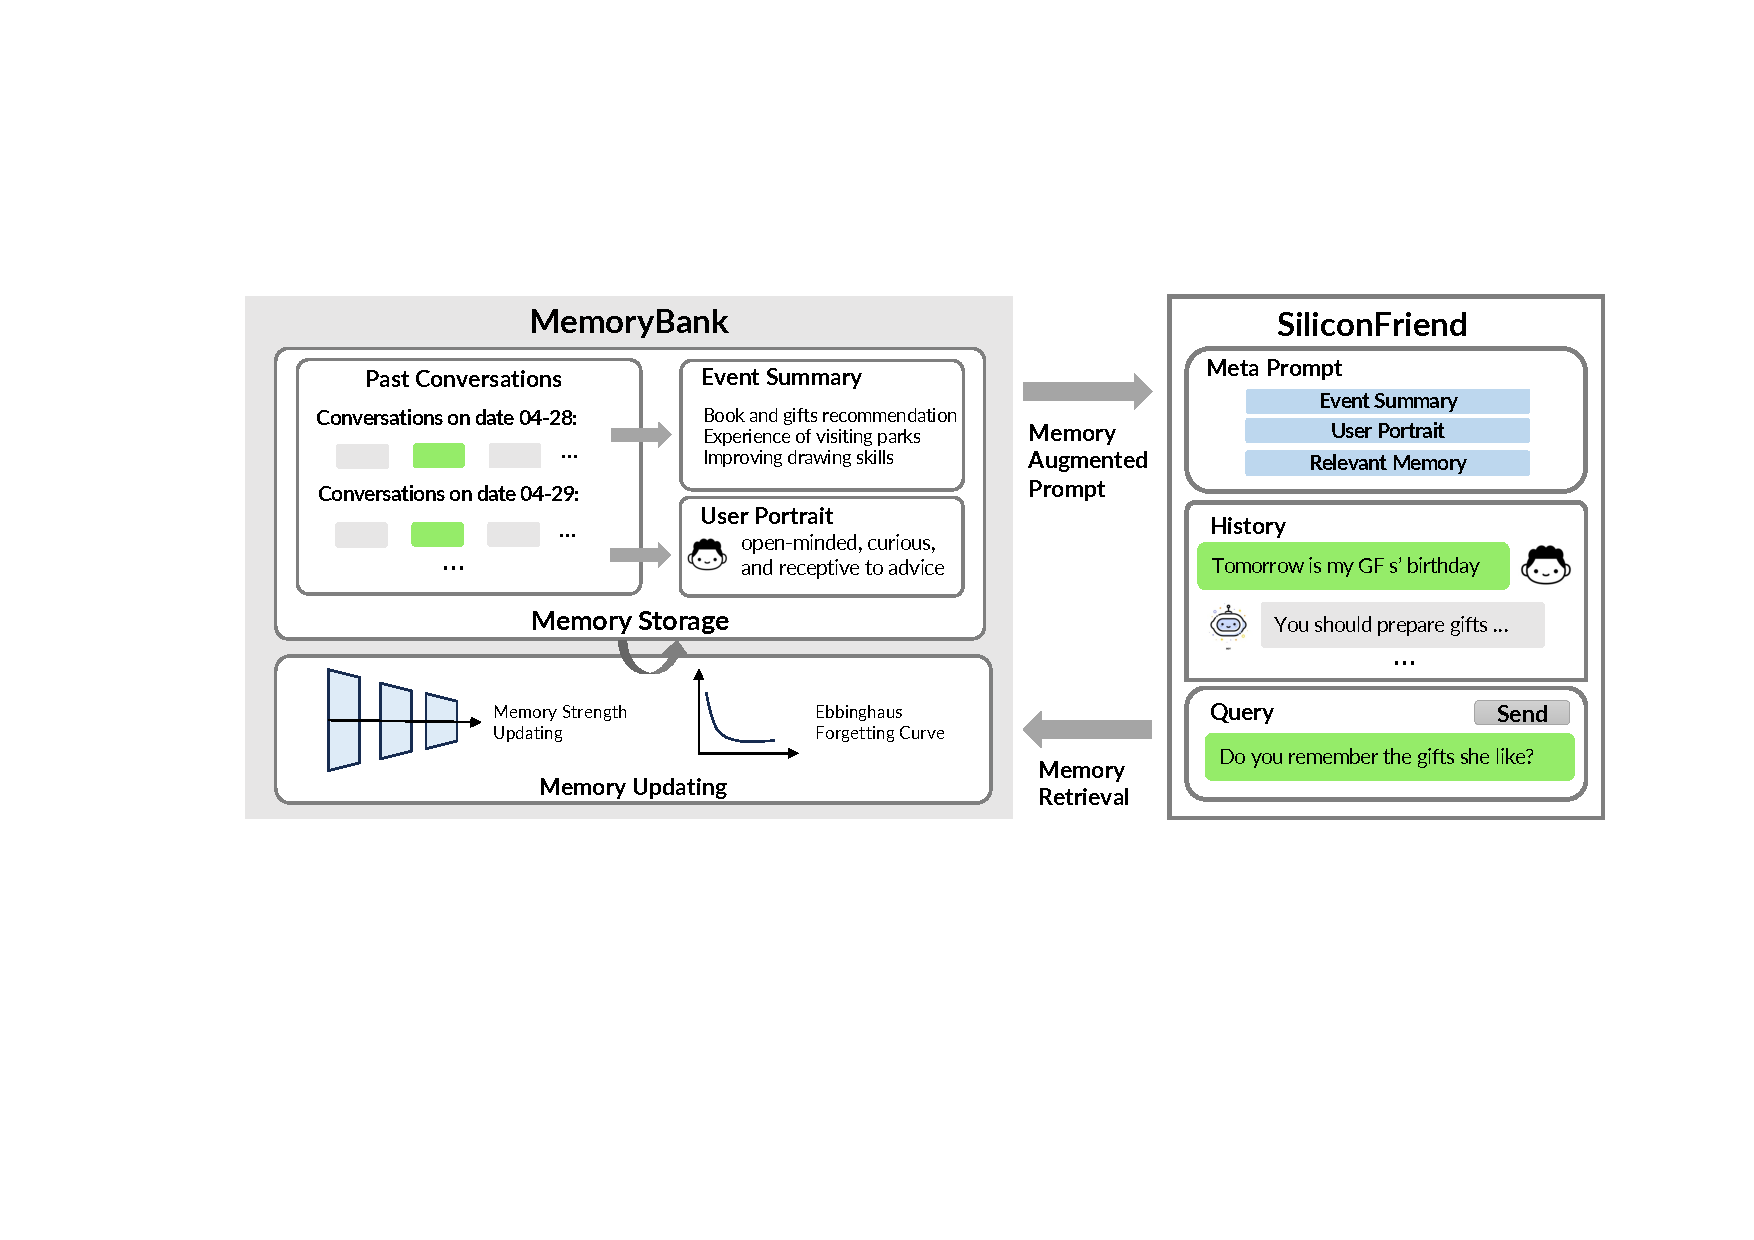
\includegraphics[width=0.99\textwidth]{figures/framework-2.pdf}
\end{center}
\caption{Overview of \method. The memory storage~(\sect~\ref{sec:memorystorage}) stores past conversations, summarized events and user portraits, while the memory updating mechanism~(\sect~\ref{sec:memory-updater}) updates the memory storage. Memory retrieval (\sect~\ref{sec:memoryretrieval}) recall relevant memory. SiliconFriend (\sect~\ref{sec:siliconfriend}) serves as an LLM-based AI companion augmented with \method. }
\label{fig:framework}
\vspace{-0.2in}
\end{figure*}

\saveSpaceSec
\subsection{Memory Storage: The Warehouse of \method}\label{sec:memorystorage}
\saveSpaceSec

Memory storage, the warehouse of \method, is a robust data repository holding a meticulous array of information. As shown in Fig. \ref{fig:framework},
it stores daily conversations records, summaries of past events, and evolving assessments of user personalities, thereby constructing a dynamic and multi-layered memory landscape.

\saveSpaceSec
\paragraph{In-Depth Memory Storage:} \method's storage system captures the richness of AI-user interactions by recording multi-turn conversations in a detailed, chronological fashion. Each piece of dialogue %( pair of conversation between AI and user) 
is stored with timestamps, creating an ordered narrative of past interactions. This detailed record not only aids in precise memory retrieval but also facilitates the memory updating process afterwards, offering a detailed index of conversational history.

\saveSpaceSec
\paragraph{Hierarchical Event Summary:} Reflecting the intricacies of human memory, \method goes beyond mere detailed storage. It processes and distills conversations into a high-level summary of daily events, much like how humans remember key aspects of their experiences. We condense verbose dialogues into a concise daily event summary, which is further synthesized into a global summary. This process results in a hierarchical memory structure, providing a bird's eye view of past interactions and significant events. Specifically, taken previous daily conversations or daily events as input, we ask the LLMs to summarize daily events or global events with the prompt ``\textit{Summarize the events and key information in the content} \texttt{[dialog/events]}''.

\saveSpaceSec
\paragraph{Dynamic Personality Understanding:} \method focuses on user personality understanding. It continuously assesses and updates these understandings with the long-term interactions and creates daily personality insights. These insights are further aggregated  to form a global understanding of the user's personality. This multi-tiered approach results in an AI companion that learns, adapts, and tailors its responses to the unique traits of each user, enhancing user experience. Specially, taken the daily conversations or personality analysis, we ask the LLM to deduce with prompts: ``\textit{Based on the following dialogue, please summarize the user's personality traits and emotions.}\texttt{[dialog]}'' or ``\textit{The following are the user's exhibited personality traits and emotions throughout multiple days. Please provide a highly concise and general summary of the user's personality}\texttt{[daily Personalities]}''.

% In summary, \method weaves together these critical components to form a more comprehensive memory management system for LLMs. It enhances their capacity to provide meaningful, personalized, and empathetic interactions over extended periods, opening up new possibilities for AI applications.

\saveSpaceSec
\subsection{Memory Retrieval}\label{sec:memoryretrieval}
\saveSpaceSec

Built on the robust infrastructure of memory storage, our memory retrieval mechanism operates akin to a knowledge retrieval task. In this context, we adopt a dual-tower dense retrieval model similar to Dense Passage Retrieval \citep{karpukhin2020dense}. 
In this paradigm, every turn of conversations and event summaries is considered as a memory piece $m$, which is pre-encoded into a contextual representation $h_{m}$ using the encoder model $E(\cdot)$. Consequently, the entire memory storage $M$ is pre-encoded into $\bm{M}=\{\bm{h}^0_{m},\bm{h}^1_{m},...\bm{h}^{|M|}_{m}\}$, where each $h_m$ is a vector representation of a memory piece. These vector representations are then indexed using FAISS \citep{johnson2019billion} for efficient retrieval.
Parallel to this, the current context of conversation $c$ is encoded by $E(\cdot)$ into $\bm{h}_{c}$, which serves as the query to search $M$ for the most relevant memory. In practice, the encoder $E(\cdot)$ can be interchanged to any suitable model.

% In our implementation of SiliconFriend with ChatGPT as the backbone, we employ LlamaIndex \cite{Liu_LlamaIndex_2022} for indexing and memory searching, leveraging the powerful embedding capabilities of ChatGPT. In contrast, for SiliconFriend built on ChatGLM and BELLE, we utilize LangChain\footnote{\url{https://docs.langchain.com/docs/}}'s indexing and memory searching capabilities, given its support for open-source embedding models and FAISS indexing.
% For language-specific implementations of open-source version of SiliconFriend, we use MiniLM \citep{wang2020minilm} as the embedding model for English, while Text2vec \citep{text2vec} serves as the go-to option for Chinese memory searching. It's important to note that these embedding models can be flexibly replaced as needed in different scenarios, even with multi-lingual models.
% In essence, \method's memory retrieval mechanism uses a versatile and efficient model that optimizes both memory storage and retrieval, enhancing the overall performance of the LLMs.


\subsection{Memory Updating Mechanism}
\label{sec:memory-updater}
% \begin{itemize}
%     \item Discussion on the inspiration from Ebbinghaus Forgetting Curve theory
%     \item  Explanation of the memory updating process and anthropomorphic behaviors
% \end{itemize} 

With the persistent memory storage and the memory retrieval mechanism discussed in \sect~\ref{sec:memorystorage} and \sect~\ref{sec:memoryretrieval}, the memorization capability of LLMs can be greatly enhanced. However, for scenarios that expect more anthropopathic memory behavior, memory updating is needed. These scenarios include AI companion, virtual IP, etc. 
Forgetting less important memory pieces that are long time ago and have not been recalled much can make the AI companion more natural.

Our memory forgetting mechanism is inspired from Ebbinghaus Forgetting Curve theory~\cite{} and follow the following principle rules\footnote{While Ebbinghaus Forgetting Curve theory includes additional features such as \emph{overlearning}~\cite{} and \emph{meaningful material effect}~\cite{}, our paper focuses on simulating the listed three principle rules.}:
\begin{itemize}
[topsep=0pt,itemsep=0pt,partopsep=0pt,parsep=0pt,leftmargin=15pt]
\item \textbf{Rate of Forgetting.} Ebbinghaus found that memory retention decreases over time. He quantified this in his forgetting curve, showing that information is lost rapidly after learning unless it is consciously reviewed.
\item \textbf{Time and Memory Decay.} The curve is steep at the beginning, indicating that a significant amount of learned information is forgotten within the first few hours or days after learning. After this initial period, the rate of memory loss slows down.
\item \textbf{Spacing Effect.} Ebbinghaus discovered that relearning information is easier than learning it for the first time. Regularly revisiting and repeating the learned material can reset the forgetting curve, making it less steep and thereby improving memory retention.
% \item \textbf{Strength of Memory.} The initial strength of a memory depends on the depth and focus of learning. Information learned with more focused attention or processed at a deeper level is remembered for longer.
% \item \textbf{Meaningful Material.} Ebbinghaus found that material that is meaningful or linked to existing knowledge is easier to retain than meaningless material. This is due to the principle of "semantic memory," where information connected to something we already know is remembered more effectively.
% \item \textbf{Overlearning.} Ebbinghaus also introduced the concept of overlearning, which suggests that continuing to learn beyond the point of initial mastery can lead to longer-lasting memories.
\end{itemize}

The Ebbinghaus forgetting curve is expressed using an exponential decay model: $R = e^{-\frac{t}{S}}$, where $R$ is the memory retention, or what fraction of the information can be retained.
$t$ is the time elapsed since learning the information. $e$ is approximately equal to 2.71828. % $e$ is the base of the natural logarithm, approximately equal to 2.71828.
$S$ is the memory strength, which changes based on factors such as the depth of learning and the amount of repetition. To simply memory updating process, we model $S$ as a discrete value and initialize it with $1$ upon its first mention in a conversation. When a memory item is recalled during conversations, it will persist longer in memory. We increase $S$ by 1 and reset $t$ to 0, hence forget it with a lower probability. 

It is important to note that this is an exploratory and highly simplified memory updating model. Real-life memory processes are more complex and can be influenced by a variety of factors. The forgetting curve will look different for different people and different types of information. 
In summary, \method~weaves together these critical components to form a more comprehensive memory management system for LLMs. It enhances their ability to provide meaningful and personalized interactions over extended periods, opening up new possibilities for AI applications.


% To further simplify memory updating mechanism, we set memory strength to 3 levels:
% \begin{itemize}
%     \item \textbf{Level-0.} Upon initial mention in a conversation, a new memory item is created and assigned Level-0. Level-0 memory  is expected to be forgotten quickly. To simulate this, we remove each memory item with a probability following the Ebbinghaus forgetting curve.
%     \item \textbf{Level-1.} If a memory item is recalled during conversation, it will persist longer in memory. We move these items from Level-0 to Level-1 and forget them with a lower probability. For simplicity, we use Ebbinghaus forgetting curve starting from day $k_1$, with $k_1$ set to 7 in our experiments.
%     \item \textbf{Level-2.} When a memory item is recalled again, it will last even longer, so we move it to Level-2. Similarly, we forget them with a probability following Ebbinghaus forgetting curve starting from day $k_2$ and $k_2$ is set to 30 in our experiments.
% \end{itemize}


% \subsection{LLM adaption}
% Integration of \method with various models (ChatGPT, ChatGLM, BELLE)

\saveSpaceSec
\section{SiliconFriend: An AI Chatbot Companion Powered by \method}
\label{sec:siliconfriend}
\saveSpaceSec

To demonstrate the practicality of \method in the field of long-term personal AI companionship, we create an AI chatbot named SiliconFriend. It is designed to serve as an emotional companion for users, recalling pertinent user memories, and understanding users' personalities and emotional states. Our implementation demonstrates adaptability by integrating three powerful LLMs that originally lack long-term memory and specific adaptation to the psychology domain.
\textbf{1) ChatGPT}~\citep{chatgpt}, a closed-source conversation model built by OpenAI, is a proprietary conversational AI model known for its ability to facilitate dynamic and interactive conversations. This model is trained on vast amount of data and further fine-tuned with reinforcement learning from human feedback. This approach enables ChatGPT to generate responses that are not only contextually appropriate but also closely align with human conversational expectations.
\textbf{2) ChatGLM}~\citep{zeng2022glm}: ChatGLM is an open-source bilingual language model founded on the General Language Model (GLM) framework. This model is characterized by its 6.2 billion parameters and its specific optimization for Chinese dialogue data. The model's training involves processing approximately one trillion tokens of Chinese and English text, supplemented by supervised fine-tuning, feedback bootstrap, and reinforcement learning with human feedback.
\textbf{3) BELLE}~\citep{BELLE}: BELLE is an open-source bilingual language model that is continuously fine-tuned from 7B LLaMA~\citep{touvron2023llama}. BELLE's feature is its automated instruction data synthesis using ChatGPT, which enhances its Chinese conversation ability.


% \begin{itemize}
% % [topsep=0pt,itemsep=0pt,partopsep=0pt,parsep=0pt,leftmargin=15pt]
% [leftmargin=15pt]
% \item ChatGPT~\citep{chatgpt}, a closed-source conversation model built by OpenAI, is a proprietary conversational AI model known for its ability to facilitate dynamic and interactive conversations. This model was trained on a comprehensive dataset and further fine-tuned with reinforcement learning from human feedback. This approach enables ChatGPT to generate responses that are not only contextually appropriate but also closely align with human conversational expectations.
% \item ChatGLM~\citep{zeng2022glm}: ChatGLM is an open-source bilingual language model founded on the General Language Model (GLM) framework. This model is characterized by its 6.2 billion parameters and its specific optimization for Chinese dialogue data. The model's training involved processing approximately one trillion tokens of Chinese and English text, supplemented by supervised fine-tuning, feedback bootstrap, and reinforcement learning with human feedback.
% \item BELLE~\citep{BELLE}: BELLE is an open-source bilingual language model that was continuously fine-tuned from  LLaMA~\citep{touvron2023llama}. BELLE's feature is its automated instruction data synthesis using ChatGPT, which enhances its Chinese conversation ability.
% \end{itemize}

% To demonstrate the adaptability of our approach, we build three versions of SiliconFriend using two open-source, bilingual LLMs (i.e., ChatGLM and BELLE) and one closed-source LLM, ChatGPT.
The development of SiliconFriend is divided into two stages.
The first stage (only for open-source LLMs) involves parameter-efficient tuning of the LLM with psychological dialogue data. 
This step is crucial as it allows SiliconFriend to offer useful and empathetic emotional support to users, mirroring the understanding and compassionate responses one would expect from a human companion.
The second stage is to integrate \method into SiliconFriend, thereby instilling it with a robust memory system. \method allows the chatbot to retain, recall, and leverage past interactions and user portrait, providing a richer, more personalized user experience.

\paragraph{Parameter-efficient Tuning with Psychological Dialogue Data:}
The initial stage of SiliconFriend's development involves tuning the LLMs using a dataset of 38k psychological dialogues. This data, parsed from online sources, comprises a range of conversations that cover an array of emotional states and responses. 
This tuning process enables SiliconFriend to understand and respond to emotional cues effectively, mimicking the empathy, understanding, and support of a human companion. It equips the AI with the ability to handle emotionally guided conversations with psychological knowledge, provide meaningful emotional support to users based on their emotional state.

To adapt LLMs to scenarios with limited computational resources, we utilize a computation-efficient tuning approach, known as the Low-Rank Adaptation (LoRA) method~\citep{hu2021lora}. LoRA significantly reduces the quantity of trainable parameters by learning pairs of rank-decomposition matrices, while keeping the original weights frozen.
Formally, consider a linear layer defined as $y = Wx$ with weight $W$. LoRA modifies this into $y = Wx + BAx$, where $W \in \mathcal{R}^{d\times k}$, $B \in \mathcal{R}^{d\times r}$, $A \in \mathcal{R}^{r\times k}$, and $r \ll \text{min}(d, k)$. This method greatly reduce amount of parameters need to be learned, which is crucial for efficiency in resource-limited scenarios. We set LoRA rank $r$ as 16 and train the model for 3 epochs with an A100 GPU. 

Noting that this stage is only conducted for open-source LLMs like ChatGLM and BELLE.
In essence, this stage lays the foundation for SiliconFriend's role as an empathetic AI companion, ensuring it can respond appropriately and helpfully to users' emotional needs.

\paragraph{Integration with \method:}
The second stage in SiliconFriend's development involves the integration of \method. This stage is vital as it equips SiliconFriend with the ability to store, retrieve past interactions and understand user portraits, thereby offering a more personalized and engaging user experience.

When it comes to memory storage, the dialogues between SiliconFriend and users are logged and updated in the memory storage, a process that is adaptable across various model backbones. 
The memory updating mechanism operates using principles inspired by the Ebbinghaus Forgetting Curve theory, allowing for a realistic and human-like memory recall process. 

During real-time conversation, the user's conversation serves as the query for memory retrieval. In practice, we use LangChain~\citep{langchain} for memory retrieval. LangChain supports open-source embedding models and FAISS indexing, making it a versatile choice.
% More specifically, for our SiliconFriend implementation that utilizes ChatGPT as the backbone, we adopt ChatGPT as the contextual embedding encoder.
% we employ LlamaIndex \cite{Liu_LlamaIndex_2022} for memory retrieval. This leverages the robust embedding capabilities of ChatGPT. 
% In contrast, 
% for SiliconFriend versions built on ChatGLM and BELLE, we turn to LangChain\footnote{\url{https://docs.langchain.com/docs/}} for memory retrieval. LangChain supports open-source embedding models and FAISS indexing, making it a versatile choice.
In language-specific implementations of the open-source version of SiliconFriend, we use MiniLM \citep{wang2020minilm} as the  embedding model for English and Text2vec \citep{text2vec} for Chinese. It is worth noting that the embedding models can be flexibly interchanged to suit varying needs, even accommodating multi-lingual models.
Upon memory retrieval, a series of information is organized into the conversation prompt, including relevant memory, global user portrait, and global event summary. Consequently, SiliconFriend can generate responses that refer past memories and deliver interactions tailored to the user's portrait.

In conclusion, these stages transform SiliconFriend from a standard AI chatbot into a long-term AI companion, capable of remembering and learning from past interactions to provide  personalized and empathetic user experience.